\documentclass[11pt, oneside]{article}   	% use "amsart" instead of "article" for AMSLaTeX format
\usepackage{geometry}                		% See geometry.pdf to learn the layout options. There are lots.
\geometry{letterpaper}                   		% ... or a4paper or a5paper or ... 
%\geometry{landscape}                		% Activate for rotated page geometry
%\usepackage[parfill]{parskip}    		% Activate to begin paragraphs with an empty line rather than an indent
\usepackage{graphicx}				% Use pdf, png, jpg, or eps§ with pdflatex; use eps in DVI mode
\usepackage{amsmath}						% TeX will automatically convert eps --> pdf in pdflatex		
\usepackage{amssymb}
\usepackage{color}
\usepackage{float}
%SetFonts

%SetFonts


\title{Exercise 1}
\author{Yapi Donatien Achou}
%\date{}							% Activate to display a given date or no date

\begin{document}
\maketitle
\section{Linear algebra}
\subsection{Matrix multiplication}
\begin{equation}
A = 
\begin{pmatrix}
2 & -1 \\
1 & 3
\end{pmatrix}
\quad 
B= 
\begin{pmatrix}
1 & 2 \\
3 & 4  \nonumber
\end{pmatrix}
\end{equation}

\begin{equation}
A*B = \begin{pmatrix}
-1 & 0 \\
10 & 14  \nonumber
\end{pmatrix}
\end{equation}

\subsection{Matrix Inversion}
\begin{equation}
 C = A*B = \begin{pmatrix}
-1 & 0 \\
10 & 14  \nonumber
\end{pmatrix}
,\quad
C^{-1}= \begin{pmatrix}
-1 & 0 \\
0.71428571 & 0.07142857  \nonumber
\end{pmatrix}
\end{equation}

\subsection{Eigen value and eigen vector}
Let a matrix $C$ be given by
\begin{equation}
C = \begin{pmatrix}
2 & -2 \\
1 & -1    \nonumber
\end{pmatrix}
\end{equation}
Its Eigen value are :
\begin{equation}
\lambda_{1} = 1, \quad \lambda_{2} = 0 \nonumber
\end{equation}


\section{Calculus}
\subsection{Gradient}
Let 
\begin{equation}\label{eq:f1}
f_{1}(x) = x^{2}+2y^{2}-xy  
\end{equation}

the gradient of $f_{1}$ is given by 
\begin{equation}
\nabla f_{1} = \left [ \frac{\partial f}{\partial x},   \frac{\partial f}{\partial y} \right ] = [2x-y, 4y-x] \nonumber
\end{equation}

\subsection{Minimum, maximum}
Find the single point $(x^{*}, y^{*})$ that minimises $f_{1}$ given by equation (\ref{eq:f1}).  $(x^{*}, y^{*})$ is the solution of 
\begin{equation}
\nabla f_{1} = \left [ \frac{\partial f}{\partial x},   \frac{\partial f}{\partial y} \right ] = [2x-y, 4y-x] = 0 \nonumber
\end{equation}
and 
\begin{equation}
(x^{*}, y^{*}) = (0,0)\nonumber 
\end{equation}

\subsection{Lagrange Multiplier}
We want dind the value of $x, y$ and $\lambda$  to minimise 
\begin{equation}
f_{1} = x^{2}+2y^{2}-xy \nonumber
\end{equation}

subjected to the constraint
\begin{equation}
g = 2x+y-22 \nonumber.
\end{equation}

To find $(x,y,\lambda)$ we define the Lagrangian by
\begin{equation}
L(x,y,\lambda) = x^{2}+2y^{2}-xy-\lambda(2x+y-22)
\end{equation}
and solve 
\begin{equation}
\begin{aligned}
\frac{\partial L}{\partial x}&= 0\\
\frac{\partial L}{\partial y}&= 0\\
\frac{\partial L}{\partial \lambda}&= 0\\
\end{aligned}
\end{equation}
for $(x,y,\lambda)$.
The solution is given by
\begin{equation}
x = 2.75,\quad, y = 16.5, \quad \lambda = -5.5 \nonumber
\end{equation}


\section{Probability}
\subsection{Conditional probability}

\begin{equation}
P(\text{card is king}|\text{card is not ace}) = \frac{P(\text{card is king \textcolor{blue}{and} card is not ace})}{P(\text{card is ace})}
\end{equation}
In a 52 cards deck we have 4 aces and 4 kings.
\begin{equation}
p(\text{card is king}) = \frac{4}{52} 
\end{equation}

\begin{equation}
p(\text{card is ace}) = \frac{4}{52} 
\end{equation}

\begin{equation}
p(\text{card is not ace}) = \frac{52}{52}- \frac{4}{52} = \frac{48}{52}
\end{equation}

\begin{equation}
p(\text{card is king \textcolor{blue}{and} card is not ace}) =\frac{4}{52} \frac{4}{48}
\end{equation}

\begin{equation}
P(\text{card is king}|\text{card is not ace}) = \frac{4}{52}
\end{equation}

\subsection{Rolling a dice}
the variance of rolling a dice with six sides is $\frac{35}{12}$ and the mean is $3.5$.
By definition, in a uniform distribution finite number of value are equally likely to be observe. If you throw a fair dice, you are equally likely to get 1,2,3,4,5,6,
that is why throwing a fair dice have a discrete uniform distribution

\section{Machine learning}
\subsection{Well posed machine learning problem}
\subsubsection{Grocery store problem}
The problem can be formulated as follow: Given a product and a location (zip code) approximate the revenue for that product. In this case:
\begin{itemize}
\item Task T: Regression (supervise learning)
\item Performance P: Root Mean Square Error
\item Experience E: Historical data of product with corresponding location and revenue
\end{itemize}


\subsubsection{Oil drilling problem}
The problem can be formulated as follow: Given a drilling technology, approximate the output oil production.
\begin{itemize}
\item Task T: Regression
\item Performance P: Root Mean Square Error
\item Experience E: historical data of output oil production per drilling technology 
\end{itemize}


\subsubsection{Self driving car}
In this case we have multiple tasks. One of then could be 
\begin{itemize}
\item Tasks T: Object recognition(Classification)
\item Performance P: $F_{\beta}$ score, Mathew correlation coefficient, 
\item Experience E: object to identify with corresponding labels 
\end{itemize}


\subsection{K-Nearest -Neighbours}
\subsubsection{Cat-dog problem}
$K = 3$, corresponds to a cats and $k=9$ corresponds to a cats

\subsubsection{Iris data set}

\begin{figure}[H] %  figure placement: here, top, bottom, or page
   \centering
   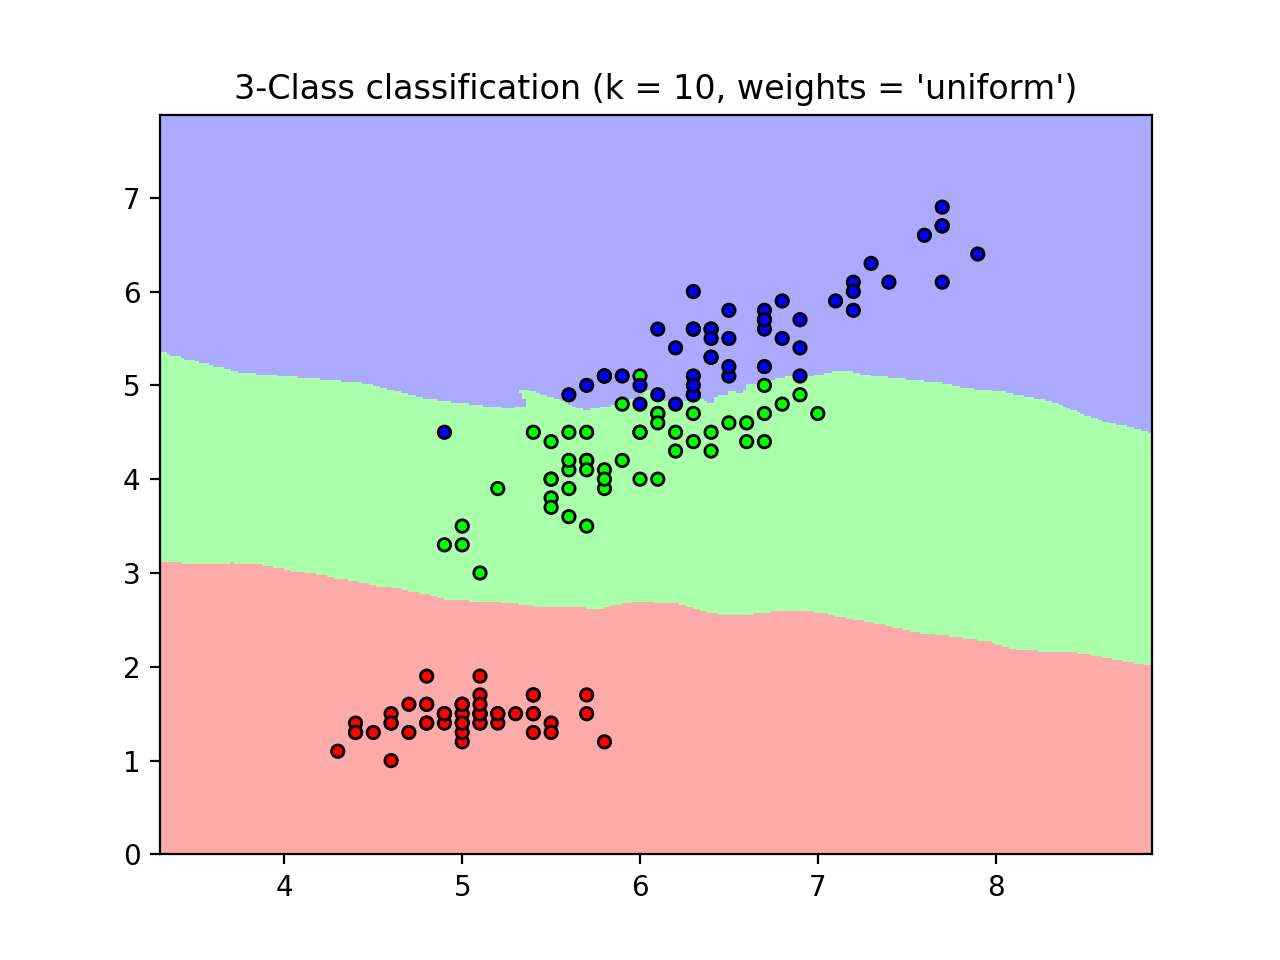
\includegraphics[width=5in]{knn10.png} 
   \caption{Classification with Iris data set. $K=10$}
   \label{fig:example}
\end{figure}

The classification result gives :
\begin{itemize}
\item red class (y=0) 50 
\item green class (y=1) 50 
\item blue class (y=2) 50 
\end{itemize}

Correct classification should be :
\begin{itemize}
\item red class (y=0) 50 
\item green class (y=1) 50 - 5 +1 = 46
\item blue class (y=2) 50 -1 +5 = 54
\end{itemize}


\subsubsection{Limitation of KNN}
The KNN algorithm uses a distance metric for classification. This works well for features with numerical values, such as petal length, petal width and so on.
For categorical features such as gender (Male, Female, Trans-sexual) it can be challenging to evaluate distance.












\end{document}  